\documentclass[a4paper,12pt]{article}

\usepackage[utf8]{inputenc}
\usepackage[czech]{babel}

\usepackage{amsmath}
%\usepackage{amssymb}
\usepackage{amsfonts}
\usepackage{fontenc}
\usepackage{graphicx}
% \usepackage{fullpage}
% \usepackage{a4wide}
\usepackage[margin=2.5cm]{geometry}
\usepackage{float}
\usepackage{array}
\usepackage{booktabs}
\usepackage{multicol}

\usepackage[dvips,unicode]{hyperref}

\author{
  René Kliment 
  ( \href{mailto:rene@renekliment.cz}{rene@renekliment.cz} )
}
\title{Matematické pětiminutovky a zajímavosti}
\date{Kompilace dokumentu: \today}

\begin{document}
 
\maketitle
 
\begin{abstract}
  Tyto úlohy jsou cíleny na středoškolské studenty jako krátká cvičení (5 - 10 minut), která mohou být rozdána na začátku hodin matematiky. Řešení většiny z nich nevyžaduje více, než zamyšlení, či tužku a papír o velikosti účtenky z velkoobchodního řetězce. Úlohy jsou zaměřeny především na přemýšlení a aplikaci základního matematického aparátu - zejména jednoduchých rovnic. Je zde určitá obecnost, která by však vzhledem k náročnosti (délce) úloh nemusela být překážkou. Cílem je donutit studenty myslet - alespoň na krátký čas a nedemotivovat je všemožnými partiemi matematiky a zároveň je přivést k vysokoškolským způsobům - "dokažte", "odvoďte", atp. v rámci látky střední školy. 
\end{abstract}

 
\section{Úlohy}

\subsection{Ruční faktorizace}

Představte si, že vás zlý čaroděj a matematik v jedné osobě uvrhl do vězení a řekl, že ven vás pustí jedině tehdy, pokud mu rozložíte libovolné přirozené číslo na součin prvočísel. K dispozici máte pouze obrovskou podlahu cely (je magická, takže tak velkou jak jen potřebujete) a váček s neomezeným počtem žetonů (něco jako Sůl nad zlato). Jak budete postupovat, pokud budete chtít uniknout dle pravidel čaroděje? Úlohu řešte s předpoklady, že umíte bezchybně počítat žetony (jeden, dva, tři, ...) a že jste dostali tak rozumně velké číslo, aby vůbec mělo cenu trávit nad tím tolik času. 
\\ \\
\textbf{Nápověda:} Z žetonů můžete skládat i jiné věci, než obrázky.

\subsection{Poměr stran papírů formátu A}
Víte, že pokud přeložíte napůl papír A\textit{n} tak, že půlíte nejdelší stranu, vznikne papír formátu A\textit{n-1}, jehož delší strana je stejně dlouhá jako kratší strana papíru A\textit{n} (tedy, delší strana A5 je stejně dlouhá jako kratší strana A4). Dále víte, že všechny papíry formátu A mají stejný poměr stran. Odvoďte z předchozích vlastností tento poměr.
\\ \\
\textbf{Návod:} Situaci si nakreslete a zapište si, co víte.

\newpage

\subsection{Střed kružnice}

Kamarád se nabídl, že vám pomůže s vaším úkolem z geometrie. Narýsoval kružnici, ale zapomněl, že měl ještě vyznačit úsečku vyzobrazující poloměr kružnice (úsečka od středu kružnice do jejího libovolného bodu). Bohužel neoznačil střed kružnice (což je další chyba) a ani nemůžete najít vpich kružítka. Máte k dispozici tužku, pravítko a kružítko. Popište, jak byste nalezli střed kružnice.
\\ \\
\textbf{Nápověda:} Využijte symetrie kružnice.

\subsection{Délka úsečky v prostoru}

Mějme v rovině, v kartézských souřadnicích, úsečku, která vede z počátku do bodu se souřadnicemi $[x; y]$. Délku úsečky spočítáme snadno jako $\sqrt{x^2 + y^2}$ - tedy jako druhou odmocninu ze součtu jednotlivých souřadnic umocněných na druhou. Vzoreček pro obdobnou situaci v prostoru s bodem o souřadnicích $[x; y; z]$ je $\sqrt{x^2 + y^2 + z^2}$. Proč, když jsme přešli do třech rozměrů zůstávají všude druhé mocniny / odmocniny a neobjevují se třetí?
\\ \\
\textbf{Návod:} Situaci si nakreslete a vzorec pro délku úsečky v prostoru odvoďte.
\\ \\
\textbf{Bonusová otázka:} Uvažujme čistě matematicky ... jak by se změnil vzoreček pro délku úsečky, pokud bychom přidali ještě jednu souřadnici (např. "u")?

\subsection{Váha}

Přišla za vámi Popelka s prosbou napočítat přesně 5894 naprosto identických kuliček hrášku. Jelikož máte chytrou váhu, není to pro vás žádný problém. Váhu zapnete, položíte na ni misku, stisknete tlačítko \textit{"nula"}, nasypete 10 kuliček hrášku, stisknete tlačítko \textit{"deset kusů"} a poté již jen sypete na váhu hrášek a sledujete na displeji počet kusů. Popelka je nicméně podezřívavá, jelikož váha vypadá jako z čínského e-shopu a chce proto vědět, podle jakého vzorce váha počet kusů spočítala. Najděte odpověď na Popelčinu otázku.
\\ \\
\textbf{Poznámka:} Váha v každém okamžiku ví \textit{kolik na ní je}. Stisk zmíněných dvou tlačítek jí umožní označit si tyto hmotnosti a zapamatovat. Ve vzorci se proto budou nalézat parametry $m_{kdyzJsemStisklNula}$ a $m_{kdyzJsemStisklDesetKusu}$, které je ovšem vhodné si pojmenovat pro přehlednost kratším názvem.
\\ \\ 
\textbf{Bonusová otázka:} Nikdy nemůžeme vážit dokonale přesně. Jak by se měla váha zachovat, co se týče zaokrouhlování? Jak "moc" (absolutní / relativní chyba) bude výsledek měření ovlivňovat to, pokud na váhu místo referenčních deseti kusů dáme o jeden méně, či více v závislosti na požadovaném váženém počtu kusů?

\newpage

\subsection{Elipsa - elipsa a kružnice}

Je kružnice elipsa? Je elipsa kružnice? Odpovězte a své odpovědi dokažte.
\\ \\
\textbf{Návod:} Určete dle definic.

\subsection{Elipsa - délka vedlejší poloosy}

\begin{figure}[H]
  \begin{center}
    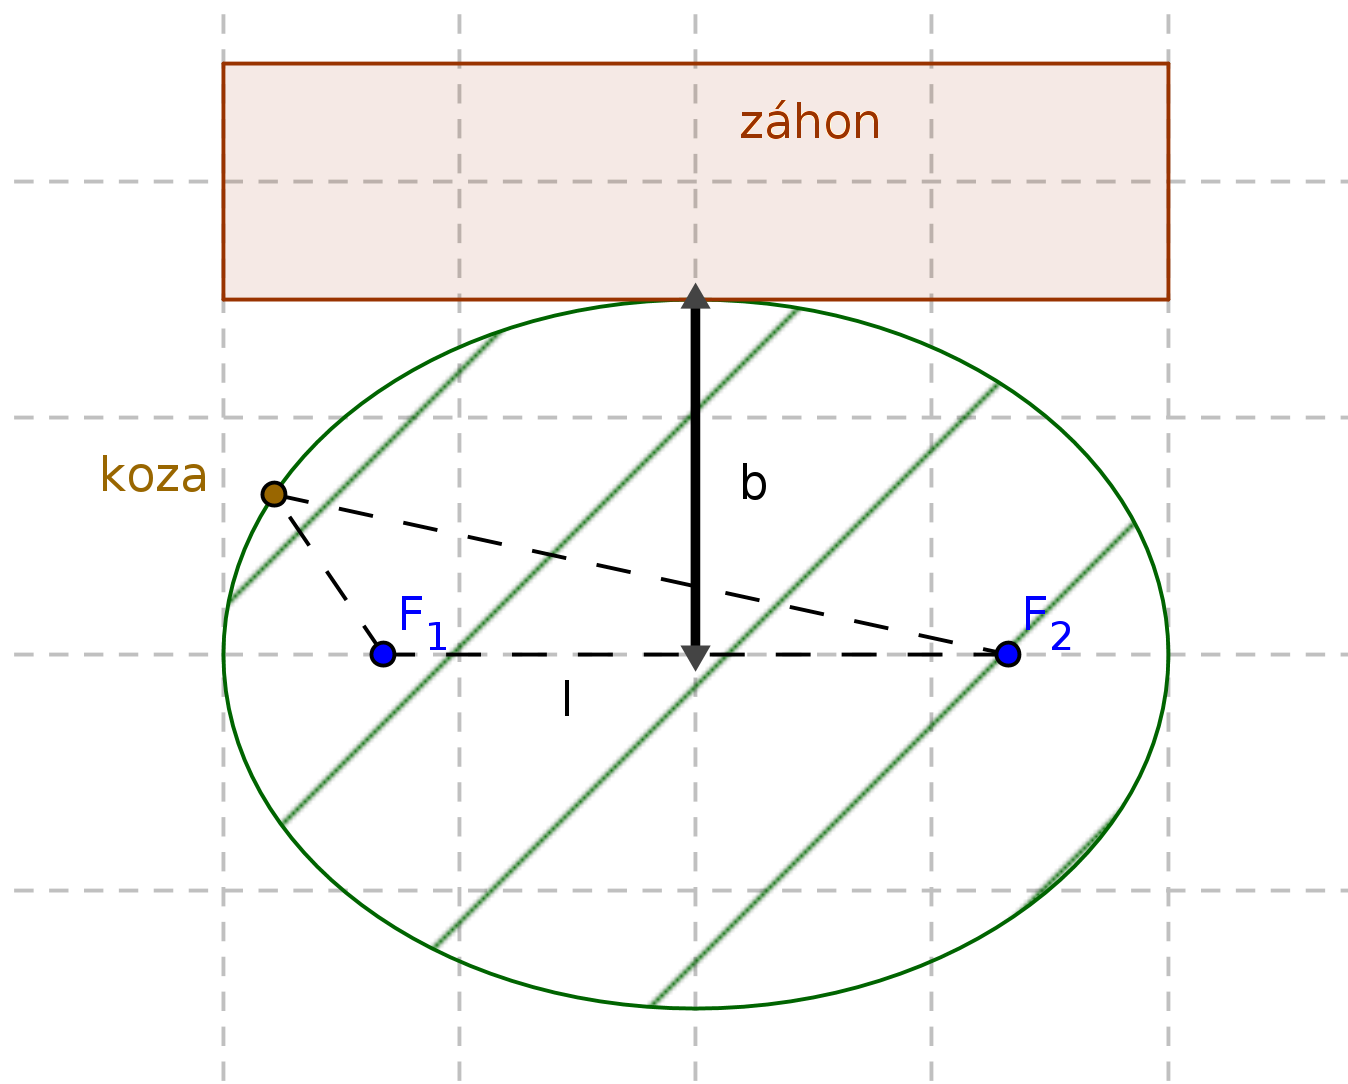
\includegraphics[width=0.4\textwidth]{data/elipsa-koza.png}
  \end{center}
  \caption{Elipsa - délka vedlejší poloosy}
\end{figure}

Malý sedlák Jan dostal od otce kozu, dva vysoké kůly ($ F_1$ a $F_2 $) a lano délky \textit{l}. Kůly zatluče do země, provazem je obejde a oba konce přiváže koze za obojek. Poraďte Honzovi, jak daleko mohou být kůly od sebe, aby koza mohla jíst trávu, ale aby nespásala záhon okrasných květin tvaru obdélníka, který je ve vzdálenosti \textit{b} od přímky spojující ohniska elipsy a jehož dvě strany jsou s touto přímkou rovnoběžné.	
 
\subsection{Elipsa - vzdálenost ohniska od středu elipsy}
 
Šílený matematik-terorista umístil v ZOO Praha k jezírku malých kachýnek výbušné zařízení. Vy jste si jako jediný návštěvník tohoto zařízení všiml. Široko daleko nikdo není a vy se proto rozhodnete bombu zneškodnit na vlastní pěst. Po odklopení krytu spatříte desku s kartézským souřadnicovým systémem, v němž je narýsovaná elipsa. Elipsa je v normální poloze (hlavní osa je rovnoběžná s osou x) a její střed leží v počátku souřadnic. Naštěstí zapomněl ve spěchu atentátník na místě návod k použití, ve kterém stojí: "pro zneškodnění propojte vodivě ohniska elipsy" a na ocejchované desce jsou napsané i délky poloos - my si pro zobecnění vystačíme s písmenky - hlavní poloosa má délku \textit{a}, vedlejší poloosa má délku \textit{b}. Za použití sponky do vlasů se chystáte bombu, jejíž časovač ukazuje pouchých 15s do výbuchu, deaktivovat. Jaké jsou souřadnice bodů, které propojíte sponkou? Řešte tuto úlohu bez předchozí znalosti vzorce, kterým spočítáte vzdálenost ohnisek od středu elipsy (která se nazývá excentricita) - odvoďte jej.
\\ \\
\textbf{Bonusová otázka:} Jaké by byly souřadnice ohnisek, pokud by střed elipsy byl v libovolném bodě o souřadnicích $[x_0; y_0]$?

\newpage

\subsection{Elipsa - konstantní součet vzdáleností}

Definice elipsy říká (něco jako), že elipsa je množina bodů v rovině, které mají konstantní součet (označíme \textit{k}) vzdáleností od dvou předem zvolených bodů - ohnisek. Dostali jste elipsu se středem v počátku kartézských souřadnic, zadanou v jejím kanonickém tvaru takto:

\begin{equation*}
  \frac{x^2}{a^2} + \frac{y^2}{b^2} = 1
\end{equation*}
\\
Zjistěte odvozením tuto konstantní vzdálenost \textit{k}.
 
\subsection{Starší bratr}

Petr je o $n$ let starší než jeho sestra. Kolikrát (minimálně, maximálně) může nastat situace, že jeho věk se rovná dvojnásobku věku jeho sestry? Kolik let každému v takovém případě bude?
 
\end{document}